%\documentclass[11pt]{article}

\documentclass[addpoints,12pt]{exam}

\usepackage[margin=2.5cm]{geometry}
\usepackage{graphicx}
\usepackage{listings}
\usepackage{xpatch}
\usepackage{color}
\usepackage{amsmath}

\makeatletter
\xpretocmd{\item@points@pageinfo}{\normalfont}{}{}
\xapptocmd{\item@points@pageinfo}{\bfseries}{}{}
\makeatother

\begin{document}
	\begin{center}
		\LARGE\scshape{Fluorescencia}
		
		\vspace{1cm}
		\large\scshape{Juan Barbosa - 201325901}
	\end{center}

	La microsco\'ia de fluorescencia es una importánte técnica de microscop\'ia ya que permite observar objetos diminutos con gran magnificación y resolución. En el caso de la fluorescencia no se usa luz transmitida sino luz reflejada (o luz emitida por la muestra).
	
	\begin{figure}[h]
		\centering
		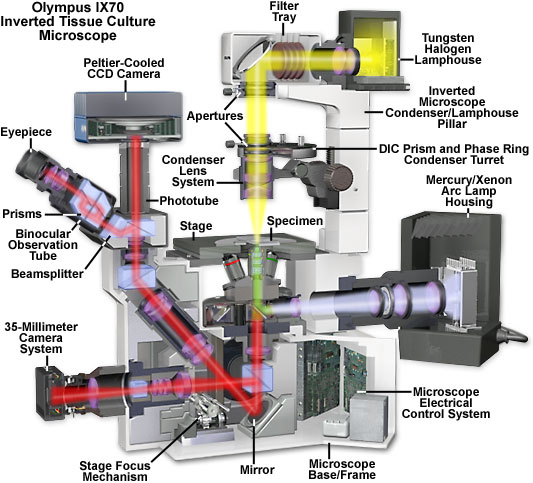
\includegraphics[width = 0.5\linewidth]{lightpaths.jpg}
	\end{figure}
	
	El esquema general del camino óptico de un microscópio de fluorescencia se muestra en la figura anterior. Un haz de luz se hace insidir sobre un filtro pasa bandas, el cual se conoce como el filtro de excitación. Posteriormente el haz pasa por el espéjo dicrócico, el cual refleja y transmite longitudes de onda específicas. Parte de la luz va en dirección
	
	
\end{document}
